\documentclass{article}
\usepackage[utf8]{inputenc}


\title{Appunti del corso di Economia dell'Innovazione - 2018/2019}
\author{Giulio Pilotto}
\date{May 2019}

\usepackage{natbib}
\usepackage{graphicx}
\usepackage{geometry}
\geometry{
	a4paper,
	total={170mm,257mm},
	left=20mm,
	top=20mm,
}

\begin{document}

\maketitle
\tableofcontents

\section{Introduzione}
Il questo corso si esplorano due prospettive Economiche: quella dell'economia dell'innovazione che si interessa delle logiche per spiegare l'innovazione, e quella del management dell'innovazione che si occupa di studiare come metterla in pratica.


\textbf{NB} $\rightarrow$  Questi appunti contengono orrori ortografici e potrebbero non risultare completi. Chiunque voglia aggiornare questo documento può rivolgersi alla repo: https://github.com/parof/eco 

\section{La teoria economica del valore}
Capire la natura della produzione permette alla politica economica di guidare l’economia su un percorso virtuoso di crescita economica (benessere economico).
Moderna confusione tra profitto (creazione) rendita
(estrazione) perché il concetto di valore oggi utilizzato
non ha un confine ben definito.
Oggi siamo incantati dal mito moderno della creazione
di valore ma se non distinguiamo tra creazione ed
estrazione rischiamo di remunerare di più la seconda
rispetto alla prima con conseguenze negative sulla
crescita economica (e la creazione di benessere)

\section{Le origini del concetto di valore}
\begin{itemize}
    \item Smith-Ricardo: Il valore è elemento critico per garantire la ri-produzione delle merci.
    \item Marx: Il valore
        partecipa alla definizione storica del metodo capitalistico di
        produzione.
    \item Neoclassici:  Il
valore c’è sempre stato e sempre ci sarà, indipendentemente dalla
forma dell’economia. 
\end{itemize}

La teoria economica comincia ad esistere in epoca borghese quando
il processo economico comincia ad essere dominato dal capitale. 
Per i fisiocratici diventa importante stabilire chi è produttivo e chi non lo è, e come si produce un intera economia.
Il concetto di \textbf{prodotto netto} diventa centrale: quella parte dell’intera
produzione sociale che eccede la ricostituzione sia dei mezzi di produzione, sia
dei mezzi di sussistenza necessari a coloro i quali, con il loro lavoro, hanno
portato all’esistenza della produzione stessa.
Con un esempio legato alla produzione agricola : il residuo che rimane dopo la riproduzione delle sementi le quali servono per garantire il processo economico, ossia lo scambio che crea mercato.



\begin{figure}[h!]
\centering
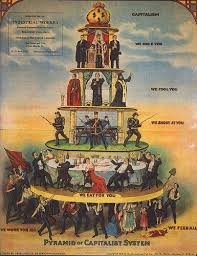
\includegraphics[scale=1.0]{images/fisiocratici.jpeg}
\caption{Pensiero Capitalista}
\label{fig:universe}
\end{figure}


\section{La scuola classica - dal valore nella terra al valore nel lavoro}
\begin{itemize}
    \item  la \textbf{rendita} è definibile come il reddito percepito in virtù della proprietà di una risorsa naturale scarsa o come la remunerazione eccedente il costo opportunità di un fattore produttivo.
    \item Il \textbf{profitto} (dalla lingua latina proficere: "andare oltre", "giovare") o lucro, in economia è l'utile (o "guadagno", indicato con G) che si ottiene da una certa attività economica (commerciale, finanziaria o produttiva).
\end{itemize}

\subsection{Smith -  prodotto netto composto da rendita e profitto}
Successivamente con l'industrializzazione della Gran Bretagna Smith arricchisce la definizione di prodotto netto come mero frutto della produzione e affermando che il valore di un bene dipende anche  a quanto lavoro serve per produrlo. 
Introduce cosi il concetto di \textbf{produttività}. Essa è legata alla divisione del lavoro quindi non dipende solo da una peculiarità del settore agricolo (la fertilità delle terre) ma dipende da caratteristiche
intrinseche al lavoro come tale, cioè dal lavoro in generale,
indipendentemente dai suoi campi d’impiego. 
\begin{figure}[h!]
\centering
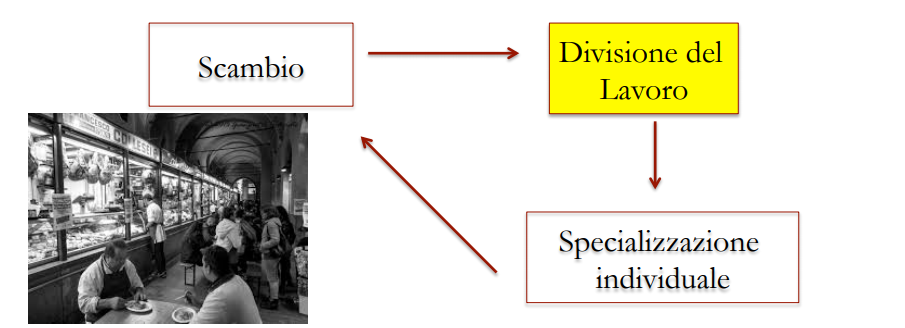
\includegraphics[scale=0.3]{images/spec_lav.png}
\caption{Smith: Mercato e prodotto}
\label{fig:spec_lav}
\end{figure}
Il \textbf{mercato} è il luogo della realizzazione degli scambi, dove cioè si ricostruisce il
nesso tra lavori individuali divisi e la reintroduzione degli uomini nella società
malgrado la specializzazione individuale.
La visione di Smith è centrata sui \textbf{rapporti sociali}. 
Il valore di scambio di una merce è il \textbf{prezzo reale}. Non il prezzo
monetario ma ciò che una merce  \textbf{realmente} vale. In origine il valore delle
merci è dato dalla quantità di lavoro necessaria a produrlo.
Per Smith, il valore della produzione non proviene da due fonti diverse (salari e
profitti) ma da un’unica fonte, il Lavoro.
\subsection{Ricardo - la distribuzione del lavoro}
Ricardo: Riprende la teoria del valore di Smith ma espande l’analisi ponendosi il problema di come il valore si distribuisce nella società sottolineando che la distribuzione non ha
nulla a che vedere con la formazione del valore. 
 Osserva il processo mercantilistico. Mette in evidenza come i processi di crescita economica non siano solo legati alla produzione, ma anche legati alla distribuzione della ricchezza nelle diverse classi sociali. Se la quantità di valore viene assorbito da una sola classe (aristocratici) ed essi hanno una rendita di valore (non producono) questo  è causa di stagnazione cioè di incapacità del sistema economico di riprodurre se stesso quando le rendite superano i profitti. 
Dibattito attuale: Le banche producono o non producono?

\subsection{Marx}
La teoria del valore in Marx ridefinisce il valore delle merci allo scopo di spiegare la
formazione del \textbf{plusvalore} non come residuo ma come reddito percepito dal
proprietario del capitale. La tesi fondamentale di Marx è che il lavoro è una merce
(fittizia) e ha un valore di mercato. Tuttavia l’oggetto dello scambio tra capitalista e
operaio non è il lavoro ma la sua capacità di lavorare \textbf{forza-lavoro}.
Per Marx il valore prodotto dall’operaio è maggiore del valore della sua forza-lavoro. 

\subsection{Verso una nuova teoria del valore - I Marginalisti}
Viene creata una visione “scientifica” del processo economico (produzione, scambio,
distribuzione del reddito).
 Sono chiamati cosi perche introducono la matematica nell' economia. Usano il calcolo infinitesimale per spiegare che succede al margine. Il valore per loro  è
 legato allo \textbf{scambio}, ovvero al mercato. Il valore dipende  dalla scarsita dei beni. Piu scarso e un bene (offerta), maggiore sara il prezzo, che definisce il valore. Il valore è soggettivo cioè è misurato dall’utilità per i \textbf{consumatore}.
Il valore viene correlato all’utilità. Rovesciamento della logica dei classici: il valore \textbf{basato sull’utilità} determina i costi di produzione e non il contrario, cioè i costi di produzione, inclusi i costi della manodopera, a determinare il valore.
Per i marginalisti, i mercati competitivi generano scambi di mercato a prezzi d’equilibrio e
quindi determinano esiti ottimali. Per ottenere esiti ottimali del processo capitalistico bisogna
eliminare tutti gli ostacoli e le imperfezioni del mercato. In questo quadro teorico la rendita
viene vista come un ostacolo (removibile) al buon funzionamento del mercato e non è più
“reddito non guadagnato”. 
\begin{itemize}
    \item In Ricardo valore = prezzo
    \item In Marx valore != prezzo (perché il valore deve essere trasformato in prezzo in quanto sono
categorie distinte. Marx usa il concetto di valore per rilevare le
contraddizioni del capitalismo).
\item Marginalisti Prezzo = utilità definita dai compratori 
\end{itemize}

\begin{itemize}
    \item Nell’economia \textbf{Classica} la rendita è l’equivalente del reddito da risorse scarse non prodotte
(ad esempio: i brevetti, le attività di corporazioni sociali come gli avvocati, le proprietà
fondiarie). La rendita, per utilizzare le parole di Marx è un diritto sul plusvalore sociale
complessivo.
\item Nell’economia \textbf{Neoclassica} i redditi corrispondono alla produttività. Non c’è rendita
(possibilità di guadagno a fronte di nessuna produzione) e nemmeno innovazione.
Se il prezzo definisce il valore dei beni allora il reddito che deriva dalla rendita è produttivo.
Non esiste, in questo quadro teorico, la categoria di reddito non guadagnato. 
\end{itemize}

Questo porta come conseguenza alla perdita del concetto di rendita.
Al giorno d'oggi per monitorare la ricchezza utilizziamo il Prodotto Interno Lordo.
In macroeconomia il prodotto interno lordo (abbreviato PIL) misura il valore aggregato, a prezzi di mercato, di tutti i beni e i servizi finali (cioè destinati al consumo) prodotti sul territorio di un Paese in un dato periodo di tempo (normalmente si usa come riferimento l’anno ma anche altri archi temporali sono usati).
Il PIL  è stato standardizzato negli anni 50. Misura la ricchezza ed e importante la decisione di cosa entra nella
misura del PIL:questa e una decisione a tavolino. 
\footnote{Riflessione sulla finanza: nella teoria  classica e neoclassica la  finanza si considerava  improduttiva, invece in questa fase attuale la finanza entra come misura importante. Le banche vengono considerate produttive.Il dibattito e comunque ancora aperto.}  

\section{Misurare la ricchezza}
I metodi contabili sono convenzioni sociali in evoluzione.
Non sono definiti da leggi fisiche e da “realtà” evidenti ma,
più semplicemente, riflettono le idee, teorie e ideologie
dell’epoca nella quale vengono sviluppati.Il PIL è influenzato dalla teoria del valore sottostante;
Il PIL è basato sul \textit{valore aggiunto} che esprime il valore
monetario di ciò che viene prodotto al netto del costo
delle materie prime o dei fattori di produzione intermedi 
Il \textbf{valore aggiunto} (anche abbreviato VA) in economia è la misura dell'incremento di valore che si verifica nell'ambito della produzione e distribuzione di beni e servizi finali grazie all'intervento dei fattori produttivi (capitale e lavoro) a partire da beni e risorse primarie iniziali.

Può essere calcolato:
\begin{itemize}
    \item dalla parte della produzione annuale
    \item dalla parte dei redditi (profitti , rendite e d interessi) annuali
    \item dalla parte della spesa, ricavata dalla domanda nei prodotti finali \footnote{Quali industrie aggiungono valore? Tutti i beni e servizi
che ricevono un prezzo sul mercato }

\end{itemize}


\section{Il concetto di Innvazione in economia}
L’aumento della produttività dei fattori è stato studiato anche dagli economisti
classici. 
\begin{itemize}
    \item \textbf{Smith}: studia “l’innovazione” come relazione tra
cambiamento tecnico, divisione del lavoro e cambiamento strutturale
dell’economia.
\item \textbf{Ricardo}: studia le conseguenze del progresso tecnico
incorporato nelle nuove macchine e distingue: effetti endogeni: la domanda aumenta perchè il prezzo delle macchine diminuisce, che ha un effetto sulla competizione tra imprese.
Effetti esogeni: la produzione di “innovazione”, cioè creazione di un
mercato di tecnologie e relativo impatto sull’occupazione. Lusso vs Beni primari.
\item \textbf{Marx} Per Marx il cambiamento tecnologico è un processo sociale nel senso che è il
risultato di una pressione competitiva e della dimensione del mercato (non è un risultato individuale)
\item \textbf{Schumpeter} Introduce il concetto di  \textbf{l'innovazione}.Il suo lavoro teorico è focalizzato sulla dinamica del cambiamento
 economico risultante dal processo di cambiamento tecnologico
di lungo periodo.
In un sistema capitalistico le imprese sono in competizione\footnote{La competizione tra le imprese è la leva all’accumulazione del capitale e alla crescita
della produttività. } e quello che dicevano i classici (Marx), è che il profitto ha una naturale decaduta per effetti di imitazione fra le imprese. Maggiore è il numero delle imprese, più aspra e la competizione e di conseguenza si ottiene una  riduzione dei prezzi e dei margini di profitto. Se la competizione cresce c'è una  caduta del saggio di profitti quindi  si attua ricerca di metodi per l aumento di produttività.
\end{itemize}
Gli elementi dello sviluppo per Schumpter:
\begin{itemize}
    \item \textbf{Innovazione}:distrugge i prodotti vecchi attraverso un processo di distruzione creatrice
    \item \textbf{L'imprenditore}:sviluppa progetti creativi affrontando il rischio, la resistenza al cambiamento e l'esitazione nel processo decisionale
    \item \textbf{Il credito finanziario}: : per introdurre un’innovazione è necessario controllare i mezzi di produzione (schei).
\end{itemize}
Per Schumpeter lo sviluppo economico ha bisogno del capitalismo come
istituzione. La competizione tecnologica determina l’evoluzione del capitalismo. 
Le imprese mantengono o migliorano la loro posizione competitiva attraverso aumenti
di produttività, cioè introducendo tecnologie più efficienti
In termini aggregati questo significa:
Accumulazione di capitale = aumento di produttività
La competizione per le tecnologie è la VERA competizione capitalistica, non quella
dei prezzi\footnote{Questo significa che ciò che veramente conta è “the competition from the new commodity, the
new technology, the new source of supply, the new type of organization, … (Schumpeter, 1943)}.
Conclusione: e condividiamo questa impostazione logica la conclusione e che le imprese competano per il prezzo, in realtà esse competono solo per avere vantaggi per le TECNOLOGIE. 

Invenzione per Schumpeter è una scoperta di nuova conoscenza. Non ha valore economico a priori. Rimane conoscenza finche non si individuta l utilita di quella tecnologia. Quado  entra nel mercato ed inventa\textbf{Innovazione}

\subsection{Cosa rende un impresa innovativa?}
Non esiste una definizione generale. Perché le caratteristiche di impresa innovativa
cambiano nel tempo. Spieghiamo questo punto.
L’impresa svolge un processo di trasformazione E dà vita a tre insiemi di attività a supporto dell’innovazione: strategiche, finanziarie , organizzative.
\begin{itemize}
    \item Le strategie d’impresa riguardano l’attività competitiva nei mercati dei
prodotti e le tecnologie da incorporare nel processo produttivo.
\item Le attività finanziarie riguardano gli investimenti necessari al cambiamento
tecnologico utile per accedere ai mercati (competitività tecnologica) e
riguardano la profittabilità attesa dell’investimento stesso.
\item Le attività organizzative riguardano la combinazione delle risorse per
ottenere un prodotto vendibile.

\end{itemize}
Queste attività hanno bisogno di un processo di apprendimento perché non è
affatto evidente come riuscire a produrre beni di buona qualità ad un prezzo
basso. 
Il processo di apprendimento è un’attività sociale, necessaria per l’innovazione.
Le sue caratteristiche sono: essere un’attività incerta, cumulativa e collettiva.

Pensiamo all’impresa innovativa: 
\begin{itemize}
    \item Deve differenziarsi dai competitors
    \item Trasformare la tecnologia e disturbare il mercato 
    \item Ridurre i costi dei prodotti già esistenti e al tempo stesso aumentarne la qualità.
\end{itemize}

\section{Le fonti dell'Innvoazione	}
\subsection{Caso PillCamera }

\begin{itemize}
	\item  \textbf{Problem Finding}: Nel 1981 Eitan Scapa, gastroenterologo israeliano convince GavrielIddan, ingegnere elettro-ottico che si occupava di controllo da remoto di missili,  a cercare una soluzione tecnologica più efficace di quelle a disposizione per esplorare il tratto interno dell’apparato digerente.
	\item  \textbf{Problem Setting}: Iddan si chiese se fosse possibile realizzare un dispositivo miniaturizzato a forma di missile senza che fosse collegato ad un cavo. Il dispositivo avrebbe avuto come “occhio” una telecamera. Problemi: qualità dell’immagine, durata batteria. (nel 1994 primo brevetto con la Applitec, ad Meron)  
	\item \textbf{Problem Solving}:  Nel 1997 Meron incontra  il dott. Swain direttore di un gruppo di ricerca in UK che stava lavorando ad un metodo di endoscopia wireless (a partire dalle microcamere disponibli sul mercato) usando frequenze a microonde. I due gruppi attivano una collaborazione e nel 1999 ottengono l’autorizzazione del comitato etico del RoyalLondonHospital per realizzare il primo esperimento su essere umano.
	Il gruppo inglese aveva una superiorità nel campo dell’anatomia umana e nella diagnostica per immagini dell’intestino mentre il gruppo israele-americano aveva conoscenze sula miniaturizzazione  dei dispositivi con basso assorbimento di energia. Nel 2001 il dispositivo ottiene il riconoscimento della FDA e GivenImaging viene quotata nella borsa NASDAQ dove raccoglie 60milioni di dollari nell’OPA iniziale.
\end{itemize}
Nasce PillCam, videocapsula da ingoiare con una piattaforma integrata (workstation, un software proprietario, una cintura da indossare con un sistema di videoregistrazione).
Fino al 2005 GivenImaging è \textbf{monopolista}. Nel 2005 Olympus introduce la sua telecamera in pillola. Altri gruppi di ricerca lavorano sul device (aggiungere gambe e pinze) GivenImaging si è \textbf{protetta} con un  patentthicket, contratti con  ospedali, corsi di formazione.

\subsection{Le fonti dell'innovazione}
Ne possiamo individuare principalmente alcune:
\begin{enumerate}
	\item \textbf{Individui}:
	\begin{itemize}
		\item \textbf{Inventore} ha una buona padronanza del settore in cui opera, che però potrebbe non
		essere l’unico campo in cui è specializzato. Tanto più l’oggetto sarà legato alla scienza e alla
		tecnologia, tanto più questo concetto è vero. L’inventore è curioso e interessato ai
		problemi; mette in discussione i modelli di pensiero dominanti (solitamente i grandi
		innovatori lo fanno).
		\item \textbf{Utilizzatore} possiede una profonda conoscenza dei propri bisogni e sono incentivati ad
		individuare soluzioni in grado di soddisfarli. Chi utilizza il bene ha
		una conoscenza superiore rispetto al suo produttore (es. snowboard). Le imprese devono
		tener conto delle potenzialità che possono provenire dagli utilizzatori.
		Le innovazioni ideate dagli utilizzatori possono anche far nascere nuovi settori come nel
		caso degli snowboard \footnote{I primi snowboard sono stati sviluppati da alcuni appassionati alla ricerca di nuovi  modi per sfrecciare sulla neve.Tom Sims realizzò il primo "ski board" in legno.Sherman Poppen creò uno "snurfer" nel tentativo di realizzare un giocattolo originale per sua figlia.Jake Burton aggiunse delle cinghie di gomma a strappo allo "snurfer" per averne un maggiore controllo.Oggi lo snowboard si è trasformato in un settore di grande rilievo, con milioni di praticanti sia in Nord America che in Europa.}.
	\end{itemize} 
	\item \textbf{Creatività di una organizzazione}:diversa perchè l'organizzazione ha delle caratteristiche sociali, che devono essere aderenti alla struttura organizzativa. Alcune sono più flessibili ed alcune più rigide.
	Al loro interno possiamo distinguere: singoli individui (es. dipendenti) e la funzione di
	Ricerca e Sviluppo (parte interna ala struttura organizzativa che svolge attività di sviluppo) \footnote{Il caso 3M (azienda americana produttrice di vari prodotti tra i quali il Post – It). Il Post – It
		nasce da un’invenzione di un dipendente dell’azienda. La 3M lavorava nel settore chimico
		come produttrice di colle, creò una colla particolare che venne usata da un suo dipendente
		per attaccare foglietti. Inizialmente il prodotto fu un insuccesso, i consumatori non ne
		capirono l’utilizzo. La 3M decise quindi di usare la strategia dell’opinion leader (influenza
		sui consumatori) regalando i post – it in luoghi pubblici per incentivare i consumatori. La
		3M è un’azienda nella quale i dipendenti hanno un tot di tempo di lavoro per fare ciò che
		vogliono; laddove individuino innovazioni verranno premiati}.
	
	\item \textbf{Relazioni  con  clienti,  fornitori, concorrenti o produttori  di  beni complementari } 
	\begin{itemize}
		\item Le relazioni di collaborazioneesterne stimolano le attività di R\&S, absorptive capacity.
		\item Le relazioni con l’Università ed enti di ricerca permettono di stare sulla frontiera tecnologica
		\item La ricerca con finanziamenti pubblici crea collegamenti tra il sistema delle imprese e il mondo della ricerca 
		\item La creazione di agenzie per il trasferimento tecnologico (parchi scientifici, incubatori) favoriscono l’accesso diretto all’esperienza scientifica (spin-off, start-up)
	\end{itemize}
\end{enumerate}

\subsection{Il ruolo della Ricerca}
\noindent
Tutti questi elementi specifici di individui e organizzazione definisco il problem setting e problem solving delle singole imprese. L'innovazione dipende dalla disponibilità di conoscienza, dall'ambiente in cui i soggetti agiscono e dalle capacita di apprendimento:pensare fuori dagli schemi aiuta a generare innovazione. Questa creatività si concretizza in disponibilità a investire in R\&S: più tutti sono innovation driven, maggiore sara disponibilità ad investire. come? con ricerca di base e ricerca applicata. la prima viene dall universita, la seconda e quando la ricerca e indirizzata a sviluppi di carattere economico.

\begin{itemize}
\item La ricerca di \textbf{Base o Pura}: essa consiste in processi orientati ad aumentare le
conoscenze dell’impresa senza considerare le applicazioni commerciali. Il suo
obiettivo è contribuire al progresso del sapere scientifico, che nel lungo termine
potrebbe poi offrire opportunità di mercato
\item La ricerca \textbf{Applicata} (effettuata sulla base delle conoscenze provenienti dalla
ricerca di base dell’impresa stessa o di soggetti esterni) è orientata all’aumento
della comprensione di un problema allo scopo di soddisfare un particolare bisogno. 
\item Per sviluppo si intende tutte le attività che consentono di applicare la conoscenza alla
realizzazione di nuovi prodotti, materiali o processi.
\textbf{Forte correlazione positiva tra quota di investimenti in R\&S di un’impresa e aumento nei ricavi e redditività}.
\end{itemize}



Ci sono due diversi approcci che l’impresa può assumere nei confronti di tale funzione:
\begin{itemize}
\item  \textbf{Science push}: in base al quale l’innovazione presenta un percorso
lineare che procede in sequenza dalla scoperta scientifica all’invenzione,
progettazione e quindi alle attività di produzione, fino ad arrivare al marketing.
Secondo questo approccio le fonti principali di innovazione sono le scoperte
scientifiche che vengono poi tradotte in applicazioni commerciali dall’impresa. La
funzione di marketing deve essere forte proprio perché il prodotto non viene
richiesto dai clienti.
\item \textbf{Demand Pull}: l’innovazione è guidata dalla domanda dei potenziali
utilizzatori, indirizzando l’impegno dei ricercatori dell’impresa verso lo sviluppo di
nuovi prodotti per cercare di rispondere ai suggerimenti o ai problemi del cliente.
\end{itemize}
La scelta tra i due approcci dipende sia dal settore in cui l'azienda opera, sia dalle dimensioni dell'azienda \footnote{In   Italia:   le   imprese   hanno   ancora   una   scarsa   propensione   agli investimenti  in  ricerca  (55,7\%  del  totale  investimenti  in  R\&D)  rispetto  al 67,5\% della Germania, all’84,5\% di Israele, 77,8\% di Giappone, 77,3\% di Cina e 70,6\% negli Stati Uniti}.

L'attività innovativa è condizionata da altri fattori:
\begin{itemize}
	\item I clienti 
	\item I fornitori \footnote{Un altro importante esempio di solida collaborazione con i fornitori italiani è UmbraGroup, che è diventata frontiere esclusivo di Boeing per le viti a ricircolo di sfere che sono installate su tutti i nostri aerei commerciali. Il Gruppo fornisce inoltre sistemi e componenti ad alta precisione con applicazione negli stessi velivoli. Nel tempo, il rapporto con Boeing ha consentito alla società di Foligno di espandersi negli USA, acquisendo una società di Seattle e aprendo una sua sede proprio in questa città.			}
	\item I concorrenti (processo di imitazione), imprese che operano nello stesso settore di riferimento.
	\item Imprese che appartengono ad altri settori produttivi.	
\end{itemize}

Spesso le imprese formano delle \textbf{alleanze} con clienti, fornitori, produttori di \textbf{beni complementari}
ed anche con i concorrenti per collaborare insieme ad un progetto di innovazione o per scambiarsi
informazioni ed altre risorse nella ricerca dell’innovazione.
Gli attori della collaborazione possono mettere in \textbf{comune risorse} quali il capitale e la conoscenza,
condividendo e distribuendo anche i rischi associati ai progetti di sviluppo di nuovi prodotti.
Le collaborazioni più frequenti coinvolgono le imprese e i propri clienti, fornitori o università locali.
Le fonti di innovazione possono essere interne (R\&S) o esterne (fornitori, altre imprese, ecc.).
La R\&S in house contribuisce a costruire la capacità di \textbf{assorbimento} dell’impresa, consentendo un
apprendimento e un utilizzo più efficaci della conoscenza acquisita da fonti esterne. La capacità di
assorbimento si riferisce all’attitudine dell’impresa a comprendere e impiegare nuove risorse di
conoscenza.
Ad oggi i grandi centri di ricerca esterni stanno sostituendo quelli interni.

\subsection{Network Collaborativi}
Il network collaborativo è un potente motore di innovazione . I network sono un
insieme di soggetti che hanno una qualche forma di legame e relazione tra di loro.
Comprende : Joint-venture, concessioni  di licenze, associazioni di ricerca, programmi, pubblico-privato, network informali.
La struttura della rete di collaborazione influenza  il flusso delle risorse , importante ruolo delle conoscenze e dell’informazione. 

I network collaborativi sono reti di imprese connesse tra loro e di istituzioni (università,
organizzazioni non profit, ecc.) operanti in determinati campi, concentrate territorialmente, dove
competono e allo stesso tempo cooperano, collegate da elementi di condivisione e di
complementarietà. La cooperazione può avvenire anche tra imprese concorrenti (es. Fiat e
Chrysler). Il concetto di network è diverso da quello di collaborazione in generale, poiché
quest’ultima prevede un \textbf{contratto lavorativo}.
Una forma di network sono i distretti industriali (es. Silicon Valley, Kilometro rosso a Milano), i
quali si contraddistinguono per le seguenti caratteristiche:

\begin{itemize}
	\item Divisione del lavoro tra imprese
	\item Condivisione delle informazioni
	\item Formazione e accumulazione di professionalità
	\item Sviluppo dei processi innovativi
\end{itemize}

\subsection{Concetto di Cluster Tecnologico}
Un altro esempio di network è il cluster tecnologico il quale è un insieme di aziende innovative che stimola la nascita di nuove imprese e attrae quelle esistenti, incentiva connessioni con fornitori e distributori sfruttando l'economia di prossimità infine attira competenze specializzate investendo in infrastrutture e servizi per la comunità.
I vantaggi di prossimità territoriale si chiamano \textbf{economie di agglomerazione}.
In essi è importante il fenomeno dello \textbf{spillover} tecnologico il quale si manifesta quando i benefici delle attività di
ricerca di un’impresa (o di altra istituzione, di un cluster o di una regione) si riversano su altre
imprese. Lo spillover tecnologico è un’azienda che nasce sulla base di una conoscenza sviluppata
da un’altra impresa; deve esserci un legame tra la base di conoscenza della nuova azienda con la
vecchia. I fattori che incidono sulla nascita degli spillover tecnologici sono:
\begin{enumerate}
	\item l’efficacia dei meccanismi di protezione della conoscenza (tanto meno ci sono meccanismi
	di protezione tanto più sarà facile prendere il know – how e creare spillover)
	\item grado di mobilità del capitale umano (possibilità di uscita dei lavoratori dalle aziende)
\end{enumerate}

\textbf{Attenzione}: La concentrazione territoriale genera anche effetti negativi 

\section{Forme e modelli dell'innvazione}

\subsection{Caso Studio Tesla Motor}
Macchina eletrica sportiva a basso impatto ambientale. Esisteva Toyota ma non era performante. incontra Musk. 
Tesla: progetto ardito (sfida al mercato automobilistico), superamento della fase della deathvalley, finanziariamente solida, capace di raggiungere gli obiettivi di mercato 

\subsection{Forme dell'innvoazione}
\begin{itemize}
	\item Innovazione di \textbf{prodotto} sono incorporate nei beni o servizi realizzati da un’impresa (Tesla Motor)
	\item Innovazione di \textbf{processo}: sono cambiamenti nelle modalità con le quali le imprese
	realizzano un determinato prodotto o servizio (es. tecniche di produzione, ecc.). Tali
	innovazioni sono spesso orientate al miglioramento dell’efficacia o dell’efficienza dei
	sistemi di produzione
\end{itemize}
Entrambe spesso sono innovazioni congiunte.
In base all’intensità e al grado di ampiezza distinguiamo (nella maggior parte dei casi si basa sulla
distanza dell’innovazione da un prodotto o da un processo preesistente):
\begin{itemize}
	\item innovazioni \textbf{radicali}: esse presentano un carattere di novità assoluta e devono
	risultare differenti in modo significativo dai prodotti e dai processi produttivi già esistenti
	(es. primo elicottero; prodotti di telecomunicazione wireless).
	\item innovazioni \textbf{incrementali}: esse non presentano caratteristiche particolarmente nuove
	o originali, possono infatti già essere note all’interno dell’impresa o del settore e consistono in cambiamenti marginali o in lievi adattamenti di soluzioni preesistenti (es.	nuova configurazione di un telefono cellulare con o senza sportellino a protezione della tastiera; modifiche elicottero).
	\footnote{Il caso delle macchine fotografiche digitali di Kodak e Sony: attività rischiosa per Kodak con un patrimonio di conoscenze sui processi chimici della fotografia (ri-orientamento strategico dell’azienda) mentre Sony possiede una sviluppata conoscenza nell’elettronica  e nello specifico nella grafica e registrazione digitale.}
\end{itemize}

In base all’effetto esercitato sulle competenze possedute dall’impresa:
\begin{itemize}
	\item innovazione competence enhancing: sono tutte quelle innovazioni che consistono in un'evoluzione della base delle conoscenze preesistenti (s. microprocessori Intel, ogni
	generazione di microprocessori incorpora un’innovazione ma fa leva sul patrimonio di
	conoscenze di Intel)
	\item innvoazione competence destroying: le innovazioni sono tali se la nuova tecnologia
	non scaturisce dalle competenze già possedute o se addirittura le rende inadeguate (es.
	passaggio dal regolo calcolatore alla calcolatrice tascabile; es. Polaroid, azienda produttrice
	di macchine fotografiche viene sostituita da un’azienda giapponese produttrice di
	macchine fotografiche digitali)
\end{itemize}

Solitamente le innovazioni competence enhancing sono sviluppate da imprese già operanti nel
settore; mentre le innovazioni competence destroying sono prodotte da imprese entranti nel
settore, ed esse sono generalmente innovazioni radicali e da queste possono nascere nuovi settori.
La maggior parte dei prodotti e dei processi è un sistema nidificato, ordinato in modo gerarchico.
La maggior parte dei prodotti e dei processi è un sistema nidificato, ordinato in modo gerarchico.
Ciò significa che l’entità considerata è un sistema di più componenti in cui, a sua volta, ciascun
componente consiste in un sistema formato da parti più piccole. Un’innovazione può implicare
una modifica dei singoli componenti (moduli, che per funzionare hanno bisogno di “parlare” la
stessa lingua e questo è possibile attraverso l’architettura), della struttura generale (architettura)
entro la quale operano i singoli componenti, o di entrambi. In base a ciò distinguiamo:
\begin{itemize}
	\item  innovazioni \textbf{modulari} prevede cambiamenti di uno o più componenti senza modifiche
	consistenti alla configurazione generale del sistema.
	\item innovazioni \textbf{architetturali} consiste in un cambiamento della struttura generale del
	sistema o del modo in cui i componenti interagiscono tra di loro.
\end{itemize}
In generale le innovazioni architetturali sono più importanti ed esse si ritengono di norma più
radicali e competence destroying (es. SYSTEM INTEGRATOR – sono aziende o specialisti che si
occupano dell’integrazione di sistemi e il loro compito è far dialogare impianti diversi tra di loro
allo scopo di creare una nuova struttura funzionale).
L’introduzione o l’adozione di un’innovazione modulare richiede all’impresa una conoscenza
limitata al componente oggetto della modifica; l’introduzione o l’adozione di un’innovazione
architetturale richiede una conoscenza più ampia dei meccanismi che governano le relazioni e le
interazioni tra le varie parti all’interno del sistema.

\section{Ciclo di vita di della tecnologia}
Le tecnologie hanno un loro sviluppo, una loro evoluzione e ciò prende il nome di traiettoria
tecnologica (l’insieme dei cambiamenti che avvengono negli anni).
Sia il tasso di miglioramento della performance di una tecnologia sia il suo tasso di diffusione nel
mercato tendono a seguire un andamento graficamente riproducibile con un curva a S.
Sebbene le due curve siano correlate fra loro (un miglioramento della performance può
incentivare ed accelerare la diffusione della tecnologia, mentre un maggior tasso di adozione può
sollecitare le imprese ad effettuare nuovi investimenti per mi

\begin{figure}[h!]
	\centering
	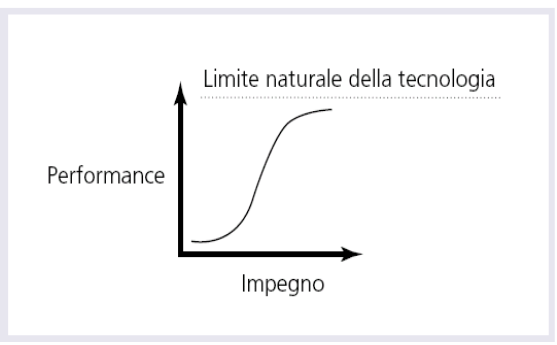
\includegraphics[scale=0.3]{images/curva_S.png}
	\caption{nella fase iniziale il miglioramento della performance è lento perché i principi di base della tecnologia sono stati compresi in maniera parziale. In seguito, quando aumenta la conoscenza della tecnologia, il miglioramento comincia ad essere più rapido. Infine, quando la tecnologia si avvicina al proprio limite naturale, la curva tende ad appiattirsi.}
	\label{fig:curva_S}
\end{figure}

Non sempre le tecnologie raggiungono il loro limite naturale.
Possono essere rimpiazzate da nuove tecnologie, definite, discontinue in quanto rispondono ad esigenze di mercato simili a quelle già soddisfatte da una tecnologia già esistente ma con una base di conoscenze completamente nuova.

\subsection{La diffusione della Tecnologia} 
Le curve a S sono usate anche per descrivere il processo di diffusione di una tecnologia. A
differenza delle curve a S della performance, le curve a S della diffusione di una tecnologia
esprimono il rapporto tra il numero complessivo di utilizzatori di una tecnologia (popolazione) e il
tempo.
In una fase iniziale, quando una tecnologia ancora poco conosciuta viene introdotta nel mercato,
l’adozione è lenta (i consumatori sono legati ad una precedente tecnologia); poi, quando gli
utilizzatori ne acquisiscono una comprensione maggiore, si diffonde nel mercato di massa facendo
aumentare il tasso di adozione (aumenta la capacità di performance della tecnologia e di
conseguenza la sua diffusione); infine quando il mercato tende a saturarsi il tasso di nuove
adozioni comincerà a diminuire.
Non sempre una nuova tecnologia si diffonde in modo veloce sebbene sia più performante della
vecchia tecnologia. Questo perché:
\begin{itemize}
	\item La nuova tecnologia potrebbe richiedere lo sviluppo di una complessa base di conoscenza;
	\item Molte tecnologie acquisiscono valore solo dopo lo sviluppo di una serie di risorse
	complementari
	\item Aspetti di carattere sociale, culturale e politico la rallentano (es. OGM)
\end{itemize}

I manager possono avvalersi dei modelli con curva a S per prevedere quando una tecnologia
raggiungerà i suoi limiti naturali, nonché affidarsi a tali modelli per decidere se e quando passare
ad una tecnologia innovativa o radicale.
Quale strumento di pianificazione la curva a S presenta però precisi limiti:
\begin{itemize}
	\item I limiti effettivi di una technolgia sono sconosciuti
	\item Cambiamenti inattesi del mercato, innovazioni nei componenti o nelle tecnologie
	complementari possono accorciare o allungare il ciclo di vita di una tecnologia.
\end{itemize}

\begin{figure}[h!]
	\centering
	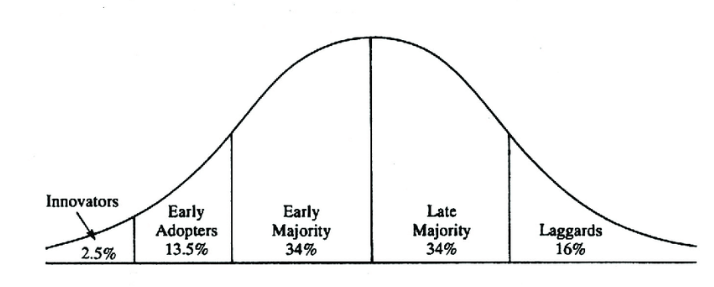
\includegraphics[scale=0.3]{images/adopters.png}
	\caption{Si studia analizzando il numero di utilizzatori di una tecnologia nel tempo}
	\label{fig:adopters}
\end{figure}

La fase di discontinuità tecnologica può modificare in maniera radicale la struttura competitiva di un settore industriale (Schumpeter distruzione creatrice).

\section{Conflitti di standard e disegno dominante}
\subsection{La concorrenza per lo standard dei pagamenti digitali}

Sqaure vs paypal
\begin{itemize}
	\item Convenienza
	\item Frode
	\item Ubiquità
\end{itemize}

Evoluzione: mobile banking

\subsection{L'affermazione di uno starndard dominante}
In breve: Diventare uno \textbf{standard} permette di sfruttare rendimenti crescenti di scala, ovvero all aumentare del volume di produzione i costi di produzione sono meno che proporzionali. Rendimenti crescente vuol dire anche che aumenta il numero di adottanti. A fronte di aumento dei profitti aumentano anche R\&S e l impresa investe anche in asset complementari. Rafforza anche cosi la posizione di cominanza della tecnologia. 

Il dominant design ha numerosi vantaggi, ma dall’altra parte porta alla perdita della
differenziazione (disomogeneità) poiché esse spinge verso l’omologazione. I fattori che portano
all’affermazione di un dominant design sono due:

\begin{enumerate}
	\item Fattori di tipo \textbf{istituzionale}: lo Stato fa una serie di interventi al fine di far affermare un
	dominant design (es. Tesla corrente alternata, UMTS nel settore della telefonia, ferrovie,
	ecc.).
	In determinati settori i benefici per il consumatore che derivano dalla compatibilità
	tecnologica degli standard sono tali da indurre gli organismi governativi a intervenire per
	imporre l’adesione ad uno standard tecnologico (es. politiche contro gli OMG in Europa).
	\item Fattori di natura \textbf{strategica}: In molti mercati le imprese convergono verso un unico disegno dominante. Uno dei motivi
	principali è che in tanti settori si manifestano rendimenti crescenti associati alla diffusione
	di una determinata tecnologia; quando cresce il numero degli adottanti, aumenta il valore
	della tecnologia.
	L’adozione e la diffusione di una tecnologia generano un margine di profitto che può essere
	reinvestito nello sviluppo e nel miglioramento della tecnologia stessa. L’utilizzo consente di
	acquisire una conoscenza più ampia e una più approfondita comprensione della tecnologia,
	permettendo di migliorare sia la tecnologia sia le sue applicazioni. Infine, un alto tasso di
	diffusione determina lo sviluppo di assets complementari concepiti per essere al servizio di
	quella tecnologia. Due fra le fonti dei rendimenti crescenti sono: effetti dell’apprendimento e
	esternalità di rete.
	
	\begin{itemize}
		\item \textbf{Effetti dell'apprendimento}  si hanno quando con l’accumulo di esperienza e di competenza
		tecnica, chi usa una determinata tecnologia impara a rendere il processo più efficiente, a
		volte sviluppando nuove soluzioni in grado di ridurre il costo degli input o l’impiego delle
		risorse utilizzate. 
		Esiste ampia evidenza empirica sulla correlazione positiva tra l’utilizzo di una tecnologia e il suo sviluppo, la sua efficacia e la sua efficienza.Questo fenomeno dell’apprendimento è rappresentabile dalla curva di apprendimento (o di esperienza), essa è una funzione del volume cumulato di produzione:
		la performance aumenta, o i costi di riducono, al crescere delle unità prodotte, solitamente
		con un tasso decrescente.
		L’economie di apprendimento ci dicono che l’utilizzo nel tempo di un bene porta ad una
		riduzione dei costi. Aumenta la performance della tecnologia con l’aumento della
		produzione.
		L’insieme di economie di apprendimento e aumento delle performance tecnologiche
		creano le basi per l’affermazione di un dominant design.
		C’è un binomio tra l’affermazione di un dominant design e la diffusione di una tecnologia
		(una tecnologia migliora la sua performance aumentando la sua diffusione).
		\item \textbf {Capacità di assorbimento} s’intende il processo di acquisizione di nuove conoscenze attraverso un’attività di apprendimento.Questo processo richiede: capacità di riconoscere valore a nuove informazioni e di saperle utilizzare in modo efficace. Ad esempio sperimentare non è una perdita di tempo in quanto si imparano procedure, organizzazione, necessità di competenze, ecc.Le imprese possono acquisire un vantaggio competitivo se per prime sperimentano e sviluppano nuove tecnologie. A livello aggregato: maggiore il numero di imprese che adottano e migliorano una tecnologia, maggiore sarà la capacità di assorbimento del sistema produttivo. E maggiori le tecnologie complementari che verranno introdotte per ulteriori miglioramenti di produttività
		\item \textbf{Esternalità della rete (o di consumo ) positive } si hanno ogni qualvolta il beneficio che deriva
		dall’utilizzo di un’innovazione aumenta al crescere del numero di utilizzatori. Aumentando
		il numero di utilizzatori della tecnologia aumenta il vantaggio (utilità). Se aumentando il
		numero di utilizzatori non aumenta l’utilità non si hanno esternalità di rete. Esse sono
		tipiche dei mercati basati su: reti fisiche (servizi ferroviari e telecomunicazioni), prodotti
		fortemente influenzati dalla presenza di beni complementari (beni accessori alla tecnologia
		legati ad essa) (Windows e le relative applicazioni software compatibili).
		Le CONOSCENZE COMPLEMENTARI (concetto diverso da bene complementare) sono legate
		allo sviluppo di un unico prodotto/tecnologia.
		È possibile rappresentare graficamente il valore offerto ai clienti da una nuova tecnologia
		considerando il valore generato dalle esternalità di rete.
		L’emergere di un dominant design fa nascere un problema di monopolio (presenza di leggi
		antitrust, le quali non condannano di per sé il monopolio, ma puniscono l’abuso di potere).
		I vantaggi di una situazione di monopolio sono dati dal fatto che esso porta maggiori profitti
		che l’impresa investirà in ReS.
		Il primo svantaggio per il consumatore, in una situazione di monopolio, è il prezzo troppo
		elevato per mancanza di concorrenza, altro svantaggio è che la qualità del prodotto non sempre è la migliore
	\end{itemize}
\end{enumerate}

\subsection{Formazione dei mercati winners-take-all}
Un’impresa in grado di affermare la propria tecnologia quale disegno dominante, di norma
guadagna enormi vantaggi e potrebbe riuscire a conservare la posizione dominante in quella
categoria di prodotto anche per il futuro. Quando un’impresa vede la sua tecnologia scelta come
disegno dominante non solo può cogliere l’opportunità di acquisire delle rendite di quasi-
monopolio nel breve termine, ma dispone anche della possibilità di “modellare” l’evoluzione del
settore e di esercitare una forte influenza sulle future generazioni di prodotto. Se un’impresa
sostiene una tecnologia che non è selezionata come standard del mercato, potrebbe esserecostretta a cedere il passo e a dover adottare la tecnologia diventata dominante, con una perdita
secca del capitale investito, dell’apprendimento e della reputazione di marca (brand equity). Nella
peggiore delle ipotesi, se non sarà in grado di adeguarsi alla tecnologia dominante, l’impresa potrà
persino essere estromessa dal mercato.
Gli economisti definiscono le arene competitive come mercati winner-takes-all (mercati in cui
predomina la tecnologia di un solo soggetto), dove il vincitore prende tutto.

\subsection{Valore stand-alone di una tecnologia}
Il valore (valore stand-alone) che una tecnologia offre ai clienti è determinato da una serie di
fattori:
Le funzioni d’uso che consente al fruitore di svolgere;
Il design e le sue qualità estetiche;
La semplicità di utilizzo.
Nei comportamenti d’acquisto dei consumatori non si considera solo la perfomance tecnologica
ma anche altri fattori.
Si deve tener conto della base di clienti, della presenza di beni complementari, ecc.
Nelle scelte strategiche delle imprese non si deve tenere conto solo della performance e dei limiti
della tecnologia ma anche di altre variabili.

\section{Tempo d'entrata}
La scelta del tempo d’ingresso (TIMING) con un nuovo prodotto in un mercato è una scelta
decisiva dal punto di vista strategico. Il timing sta assumendo sempre più importanza (modifica nei
gusti dei consumatori).
Ci sono tre diverse tipologie di strategia da poter adottare:
\begin{itemize}
	\item \textbf{First Mover} (primo entrante o pioniere) imprese che entrano per la prima volta nel
	mercato con un nuovo prodotto basato su competence destroying (innovazione
	radicale).
	\item \textbf{Early Follower} (primi inseguitori), sono imprese che entrano, successivamente, al
	first mover, ma ancora in una fase di incertezza (non si sa se il prodotto riuscirà ad
	affermarsi); il numero di imprese è maggiore rispetto ai first mover;
	\item \textbf{Late Entrant} (entranti ritardatari), imprese che entrano quando il prodotto o la
	tecnologia si è già affermata.
\end{itemize}

\subsection{Vantaggi di un First mover}
\begin{itemize}
\item Fedeltà di marca (brand loyalty), l’impresa guadagna una reputazione di lunga durata quale
leader in una determinata tecnologia. Tale status permette all’impresa di rafforza la sua
immagine, estendere la propria brand loyalty e allargare la quota di mercato anche dopo
l’introduzione di prodotti analoghi da parte dei concorrenti. Se le caratteristiche della
tecnologia sono difficili da imitare, la posizione di leadership tecnologica determina per
l’impresa una rendita da monopolio sostenibile nel tempo. Anche quando le caratteristiche
sono imitabili, il first mover ha comunque l’opportunità di costruire una relazione di fiducia
con il cliente prima dell’ingresso sul mercato dei concorrenti.
\item Diritto di opzione su risorse scarse (tutti i fattori necessari a sviluppare una certa
produzione, possono essere tangibili e non), le imprese che entrano per prime godono di
un vantaggio di prelazione o di opzione nell’acquisizione di risorse scarse. I concorrenti
potrebbero essere esclusi dall’accesso a tali risorse.
\item Sfruttamento switching cost dell’acquirente , una volta adottata una determinata
tecnologia il passaggio a una diversa comporta spesso dei costi per il cliente, definiti
switching cost. In particolare quando il prodotto è complesso, il cliente dovrà impegnare
parte del suo tempo per acquisire familiarità con esso. Tale investimento diventa uno
switching cost che scoraggia il potenziale acquirente dal passaggio a un prodotto
alternativo.
\item Vantaggi dei rendimenti crescenti , in un settore con pressioni competitive che spingono per
l’adozione di un progetto dominante, la scelta del timing degli investimenti nello sviluppo
di una nuova tecnologia può essere decisiva. Il first mover ha vantaggi (es. prezzo) poiché
avrà una massa di clienti superiore alle imprese che entrano successivamente.
\end{itemize}
Tutti questi vantaggi modificano la concorrenza tra first mover e imprese entranti
successivamente. L’importanza di tali vantaggi dipende dal settore di riferimento (es.
mercato della moda la brand loyalty è molto importante; nel caso di prodotto tecnologico
tale fattore non ha invece molta importanza).
\subsection {Svantaggi First Mover}
Esistono anche dei validi motivi per non entrare troppo presto in un mercato. Gli svantaggi del first
mover sono:
\begin{itemize}
\item Alti costi di ricerca e sviluppo , per essere leader nel settore l’impresa deve investire più
degli altri nella ReS. Il first mover per poter arrivare sul mercato con una determinata
tecnologia ha dovuto investire le proprie risorse in più progetti, poiché non sapeva quale
fosse la tecnologia migliore. I late entrant non devono investire in più progetti proprio
perché già sanno qual è la tecnologia su cui puntare.
\item Sviluppo dei canali di fornitura e distribuzione , tanto più il prodotto è innovativo tanto più
il first mover avrà difficoltà, non solo nella produzione, ma anche nella sua distribuzione al
cliente, per l’assenza o l’inadeguatezza del sistema di fornitori o distributori (es. Telecom,
first mover nella telefonia italiana)(es. Apple store, usato per la distribuzione hi-tech).
\item Sviluppo delle tecnologie abilitanti e dei beni complementari , le tecnologie abilitanti
servono per far funzionare la tecnologia principale (es. batteria dei cellulari).
\item Incertezza nelle condizioni della domanda , tanto più il prodotto è innovativo tanto più si
rischia il fallimento del prodotto (innovazioni di insuccesso) poiché non è detto che il
cliente lo capisca.
\item Incumbent inertia: i nuovi entranti sono in grado di adottare processi
produttivi più innovativi/superiore efficienza
\end{itemize}
Per quanto riguarda i follower (early follower e late entrant) i vantaggi del first mover sono loro
svantaggi; al contrario gli svantaggi del first mover sono i loro vantaggi.

\subsection{Fattori che determinano la strategia d’entrata ottimale}
\begin{itemize}
	\item Soddisfare una domanda già manifestata.
	Nella decisione il fattore discriminante sarà il rischio (gap tra rischio e benefici). Il fatto di
	sapere che cosa vuole il cliente abbassa il rischio di insuccesso. Tanto più il first mover
	immetterà sul mercato un prodotto che risponde alle esigenze del cliente tanto minore
	sarà l’incertezza e il rischio.
	\item Miglioramento rispetto alle soluzioni tecnologiche precedenti.
	Si ha nel caso in cui la nuova tecnologia soddisfa una domanda già esistente. Anche in
	questo caso il rischio è minore.
	\item Presenza di tecnologie abilitanti e di supporto.
	Se il first mover entra in mercati in cui ci sono già tecnologie abilitanti e di supporto il
	rischio è basso.
	\item Presenza di beni complementari (o di facile sviluppo).
	Se il valore dell’innovazione dipende dalla disponibilità e qualità dei beni complementari,
	saranno le caratteristiche di questi a determinare le probabilità di successo dell’entrata nel
	mercato. Se tali beni già esistono è più facile l’ingresso per il first mover.
\item 	Presenza di barriere all’entrata.
	La barriera all’entrata si ha quando la nuova entrante deve sostenere costi per entrare nel
	mercato maggiori delle imprese che già operano in esso. In una situazione di barriera
	all’entrata il first mover è incentivato ad entrare poiché ottiene un vantaggio rispetto ai
	follower (la barriera lo protegge dai concorrenti). È allo stesso tempo anche un rischio
	poiché il first mover deve sostenere elevati costi, laddove il prodotto non sia di successo ciò
	determinerebbe una perdita.
\item 	Presenza di rendimenti crescenti da adozione.
	Tanto più sono elevati i rendimenti crescenti tanti più conviene adottare una strategia di
	first mover.
\item 	Sostegno finanziario alle strategie di ingresso.
	Tanto più elevate sono le risorse finanziarie dell’impresa tanto più essa può sostenere il
	rischio.
\item 	Reputazione dell’impresa e incertezza del mercato.
	Oltre alle risorse finanziarie, anche la reputazione e la credibilità dell’impresa possono
	influenzare la scelta d’ingresso nel mercato. La reputazione dell’impresa invia forti segnali
	relativi alle possibilità di successo di una nuova tecnologia. Maggiore è la reputazione
	dell’impresa tanto minore sarà il rischio di insuccesso.
\end{itemize}

\begin{figure}[h!]
	\centering
	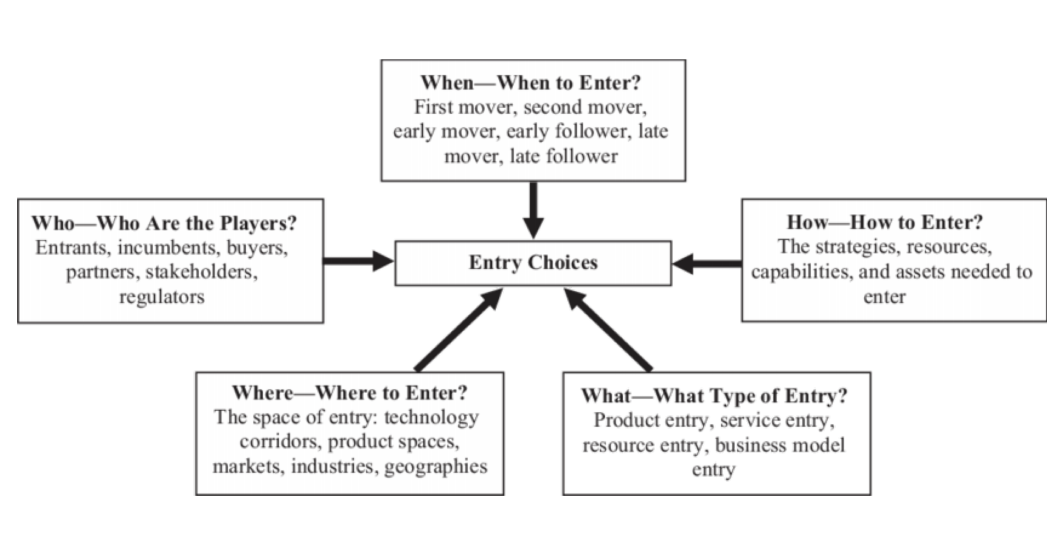
\includegraphics[scale=0.4]{images/Entry_choice.png}
	\caption{When you move first?}
	\label{fig:entry_choice}
\end{figure}

\subsection{First Movers vs Follower}
Se la tecnologia proposta dal first mover è performante ed è difendibile (alte barriere, bassa
imitabilità) conviene una strategia di first mover.
Se invece la tecnologia è incerta, facilmente imitabile e ci sono basse barriere all’entrata è
preferibile essere follower.
Sulla strategia da perseguire incide anche la dimensione e la disponibilità di risorse dell’impresa.
Già nella fase della ReS si può determinare la strategia d’ingresso. Le fasi della ReS sono:
Ricerca di base;
Ricerca applicata;
Sviluppo;
Capacità di assorbimento.
Se si decide di adottare una strategia di follower l’impresa investirà nella fase legata alla capacità
di assorbimento (la ricerca di base la prendi dal first mover e la inserisce nell’organizzazione).
Caso contrario, quando la strategia è di first mover, l’impresa investirà in ricerca di base.
È nella fase della progettazione della funzione di ReS che le imprese stabiliscono la strategia da
adottare.

\subsection 
{FMA nel mercato Abilitato da Internet}

\section{Definizione dell'orientamento strategico}
\subsection{Come si contruisce nua strategia basatas ull'innovazione?}
Per analizzare una strategia è necessario:Valutare la posizione competitiva dell’impresa,definire l’orientamento strategico per il futuro.
\begin{figure}[h!]
	\centering
	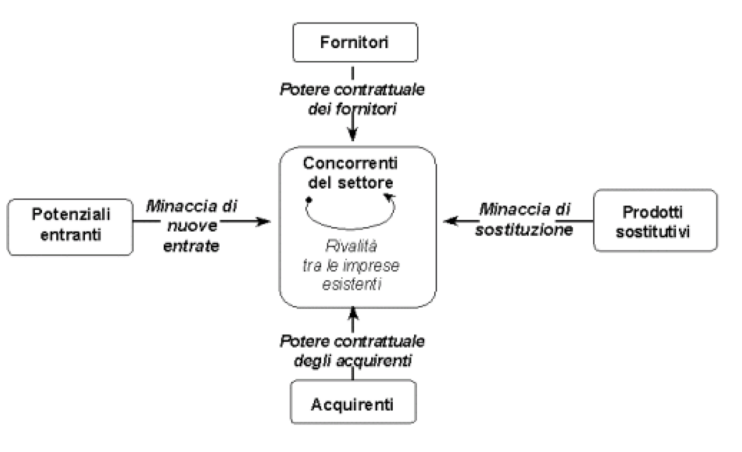
\includegraphics[scale=0.4]{images/Porter.png}
	\caption{Il modello delle cinque forze di Porter (1980)
		per la valutazione della posizione competitiva
		dell’impresa. Modello
		utilizzato per
		valutare:
		Attrattività di
		un settore e
		L’ambiente
		competitivo
		di un’impresa}
	\label{fig:Porter}
\end{figure}

Il grado di competitività  dipende:
\begin{itemize}
\item Numero e dimensioni dei concorrenti
\item Differenziazione dei concorrenti
\item Condizioni della domanda
\end{itemize}
Minaccia di entranti potenziali dipende:
\begin{itemize}
	\item Attrattività del settore (es. redditività)
	\item Barriere all’entrata (scoraggiano l’ingresso)
	\item Strategie di penetrazione (es. partnership)
\end{itemize}
Il potere contrattuale dei fornitori
dipende:
\begin{itemize}
	\item Numerosità dei fornitori
	\item Differenziazione dei fornitori
	\item Switching cost per passare ad un
	altro fornitore
	\item Integrazione verticale a monte da parte degli acquirenti
\end{itemize}

La minaccia dei prodotti sostitutivi:
\begin{itemize}
	\item Similarità della loro funzione con quella
	dell’impresa
	\item Prezzo relativo dei beni sostitutivi
\end{itemize}

Sesta forza: i beni complementari
La disponibilità, qualità, prezzo dei complementi
influenzano le opportunità e le minacce per le
imprese del settore.

\subsection{Analisi stakeholders}

\begin{figure}[h!]
	\centering
	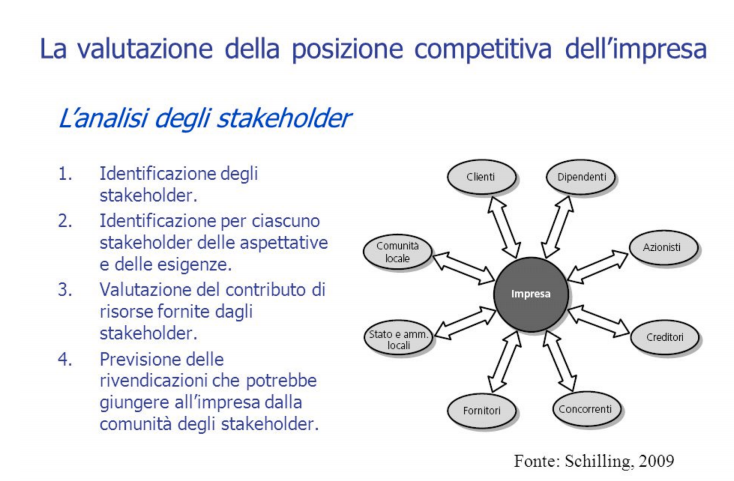
\includegraphics[scale=0.4]{images/stakeholders.png}
	\caption{Analisi stakeholders di Porter}
	\label{fig:Porter2}
\end{figure}

\subsection{Analisi del cambiamento interno }
Ciascuna attività può essere valutata in base alla sua capacità di contribuire alla creazione del valore complessivo dell’impresa Identificati i punti di forza e debolezza, il management dovrà valutare quali sono i fattori che garantiscono un vantaggio competitivo sostenibile.
Su cosa si basa un vantaggio competitivo sostenibile?Risorse rare, di valore, durevoli, difficilmente imitabili

\subsection{Le competenze distinitve (core competencies)}
Le \textbf{competenze distintive} distinguono un’impresa sotto il profilo strategico.Sono il risultato di processi di apprendimento e di accumulazione di conoscenzeSono proprietà emergentidal processo di problem-solving. Sono la risultato di integrazione di parti di conoscenza.

Il concetto di competenza è rilevante perché:
\begin{itemize}
\item Le imprese possono essere definite rispetto al loro insieme di competenze
\item Le competenze sono firm-specific
\item Le imprese differiscono per quantità e varietà di competenze
\item Le competenze possono essere un elemento di vincolo nella possibilità di assorbire processi
\end{itemize}
\subsubsection{Le dimensioni delle competenze}
\begin{enumerate}
\item Dimensione \textbf{inerziale} (path-dependence): l’inerzia dipende dalla ripetizione di ciò che si conosce. Gli sviluppi futuri non vengono considerati.                  
Trappola delle competenze, che cosa manca?
Le \textbf{meta-competenze}: sono la dimensione dinamica delle competenze, cioè la capacità di adattamento dell’impresa. Sono la capacità di apprendimento e di creazione di nuova conoscenza.
Le meta-competenzesono fondamentali per lo sfruttamento e l’esplorazione della conoscenza
\item Dimensione del \textbf{contesto tecnologico}:se il cambiamento tecnologico è molto rapido produce una nuova frontiera di sfide (tecnologie che distruggono o rafforzano competenze).

\end{enumerate}
Le competenze distintive definiscono \textbf{l’intento strategico} e coinvolgono tutti i livelli organizzativi dell’impresa. Tale obiettivo solitamente ha un orizzonte temporale di lungo periodo e scandisce tutte le tappe intermedie per poter essere raggiunto.L’intento strategico è importante per non confinare l’impresa ai mercati acquisiti (lock-in) ed esplorare nuovi mercati, modellare le aspettative dei mercati futuri, ridiscutere il rapporto prezzo-performance.

\section{Scelta dei proegtti di innovazione}
\subsection{Caso Bugs Lab}
Bug Labs is a technology company headquartered in New York City that began by developing and sellingopen-source hardwareperipherals forrapid prototypingof electronic devices. The company, founded in April 2006,[1]developed a Lego-like hardware platform that technology enthusiasts, hobbyists and engineers used to create their own digital devices. Currently, the company develops software and firmware in order to connect devices to the internet, and has partnerships with several Fortune 100 companies, including mobile phone operators, to ignite invention of new kinds of wireless devices.Bug Labs recently announced a new data sharing utility for the Internet of Things calleddweet.io.dweet.iois a simple and lightweight messaging service for devices. It requires no setup or sign in, just publish and go. Send data from your thing to the cloud by "dweeting" it with a simple HAPI-REST web API. You can also play with dweet.iousing theirAPI console.
Nel 2006, i fondatori di Bug Labsdecidono di creare l’azienda convinti che ci siano opportunità economiche nella “coda lunga” del mercato dei dispositivi elettronici.Le grandi imprese di elettronica sono, per lo più, orientate al mercato di massa o al segmento di fascia alta di clienti, per poter coprire gli alti costi di sviluppo e di personalizzazione dei prodotti.L’idea di Bug Labsè invece quella di centrare il business sui micro-segmenti di mercato con prodotti modulari, ciascuno con differenti funzioni, che il cliente potrà combinare –come fosse un lego -per realizzare il dispositivo desiderato.Il mercato di riferimento è difficile da stimare ex ante e rende impraticabile per l’azienda l’adozione di metodi tradizionali per la valutazione di progetti innovativi.


\subsection{Valutazione dei progttei d'innovazione}
Ampia varietà di metodi, da strumenti informali a tecniche sofisticate, basati su dati qualitativi oppure fondati su ipotesi rigorosamente quantitative.Il primo importante passo sta nella valutazione del razionamento del capitalenelle decisioni di investimento Tendenzialmente si usa un mix di strumenti per identificare opportunità e rischi di un progetto innovativo

\subsubsection{Budget di sviluppo per settore }
a maggior parte delle imprese dispone di risorse limitate (vincoli di capitale). Questo determina la selezione di progetti innovativi e/o la necessità di trovare capitale esterno (crowdfounding)La selezione viene fatta adottando metodi di “razionamento” del capitale:prima si stabilisce un budget per le attività di R\&S e poi si definisce una classifica dei progetti per scegliere quelli da finanziare.Tendenzialmente,il budget viene fissato in termini di una quota determinata del fatturato dell’anno precedente.Tale percentuale è stabilita basandosi su parametri di settore (industrybenchmark) oppure su indicatori storici rilevati dalle performance aziendali (historicalbenchmark).

\subsection{Metodi quantitativi per la scelta dei progetti}
\subsubsection{Le tecniche di attualizzazione dei flussi di cassa}
\begin{itemize}
\item Tecnoche di attualizzazione dei flussi di cassa:
 Valore attuale netto = i flussi di cassa attesi in entrata sono attualizzati
 e confrontati con il valore attuale dei flussi monetari in uscita
\item Il VAN è un metodo per prendere decisioni finanziarierelativamente
ad un progetto combinando il valore attuale dei suoi benefici e il
valore attuale dei suoi costi. L’attualizzazione viene effettuata
utilizzando un tasso di sconto che tiene conto del costo
opportunità della moneta, in un arco di tempo definito. Il VAN
permette di calcolare il valore del beneficio netto atteso dal progetto
come se fosse disponibile nel momento in cui la decisione di
investimento viene assunta.
\item  Il criterio del VAN:
Una decisione d’investimento impone una scelta.
Occorre scegliere l’alternativa con il VAN più elevato.
(Questa opzione significa scegliere l’alternativa che riceve maggior
denaro oggi).
Altrimenti:
E’ necessario accettare o rifiutare un progetto.
Accettare progetti con VAN positivo: equivale a ricevere un VAN
positivo
Rifiutare progetti con VAN negativo: equivale a tutelare la
ricchezza degli investitori
\item Il tasso interno di rendimento (TIR o IRR: internal rate of return)
costituisce il tasso di attualizzazione dei cash flow per cui il valore attuale
dei flussi in ingresso eguaglia il valore attuale dei flussi in uscita.
È il tasso di attualizzazione che rende il valore attuale netto
dell’investimento pari a zero.
\item Relazione grafica tra VAN e TIR. Siccome il TIR è il tasso di
attualizzazione che rende nullo in VAN di un investimento, il
grafico aiuta ad individuare il TIR del progetto
\end{itemize}
Le tecniche di attualizzazione dei flussi di cassa offrono particolari
vantaggi:
- forniscono delle stime finanziarie di progetti alternativi
- considerano in modo esplicito i tempi dell’investimento e il valore
finanziario del tempo
ma hanno anche dei limiti:
- potrebbero essere ingannevoli e dipendono dall’accuratezza delle
previsioni iniziali dei flussi di cassa
- potrebbero non essere in grado di cogliere l’importanza strategica di
una determinata decisione di investimento.
\subsubsection{Il metodo delle opzioni reali}

La dimensione finanziaria non esaurisce la valutazione della decisione
	di investimento nello sviluppo di un nuovo prodotto.
	È una tecnica di valutazione che applica il modello del diritto di opzione
	su titoli azionari a un progetto di investimento.
	Funzionamento dell’opzione reale nel mercato finanziario:
	• Un investitore lancia un’opzione di acquisto (call option) che gli
	riserva il diritto di acquistare l’azione in futuro entro o ad una certa
	data (maturity) ad un prezzo prefissato (prezzo d’esercizio o strke
	price). Se in futuro il valore dell’azione supera il prezzo d’esercizio, il
	possessore dell’opzione potrà far valere il proprio diritto e
	acquistare l’azione.
		Per esempio nel caso di un programma di R\&S:
	\begin{itemize}
	
		\item il costo del programma di R\&S può essere considerato il prezzo di
		un’opzione di acquisto (call option)
		\item il costo dell’investimento futuro per sostenere e finanziare il
		programma rappresenta il costo di esercizio
		\item il ritorno dall’investimento in termini di valore attuale dei flussi di
		cassa attesi dal progetto di R\&S corrispondono al valore di
		un’azione acquistata con diritto di opzione
	\end{itemize}
	Il metodo delle opzioni reali è utile soprattutto nella valutazione di
	investimenti ad alto grado di incertezza, come per esempio i progetti
	innovativi.
	Tuttavia presentano non pochi limiti, poiché molti progetti innovativi
	non si conformano alle ipotesi rigorose sotto il profilo formale dei
	mercati finanziari a cui il modello si ispira (il valore di una stock option è
	indipendente dal comportamento del detentore del diritto di opzione,
	ma invece il valore di un investimento in R\&S è condizionato dalle
	competenze possedute dall’impresa, dalle risorse complementari, dalle
	sue strategie).

\subsection{Metodi Qualitativi}
\begin{itemize}
	\item Domande-filtro - Sono impiegate per approfondire e valutare le principali dimensioni che
	influenzano la scelta, quali:
	\begin{itemize}
		\item il ruolo dei clienti (mercato, utilizzo del prodotto, compatibilità e facilità
		d’uso, distribuzione e strategie di prezzo)
		\item il ruolo delle capacità e delle competenze organizzative (capacità e
		competenze possedute e prospettiche, capacità dei concorrenti)
		\item i tempi e i costi del progetto
	\end{itemize}
Una volta completata la check-list, il management può avviare una
discussione aperta attorno al progetto oppure creare un sistemi di
punteggi per ogni risposta per ponderare la rilevanza di ogni singolo
fattore.
Questa tecnica pur non fornendo risposte definitive sull’opportunità del
finanziamento di un progetto consente di affrontare un ampio ventaglio di
questioni critiche per la decisione finale.

\item La mappa del portafoglio in R\&S: identificazione del mix desiderato di
progetti e definizione dell’allocazione delle risorse.

\item Il metodo Q-Sort (ordinamento qualitativo): selezione qualitativa è una
semplice tecnica di classificazione di oggetti o idee in base ad una serie
di parametri
\begin{itemize}
	\item le idee o le varianti di progetto sono descritte in una carta
	\item per ciascuno dei parametri selezionati, le carte sono ordinate in
	base alla capacità di risposta di ciascun progetto
	\item una serie di round di confronto fra le differenti classifiche,
	accompagnati da una discussione fra i partecipanti, dovrebbe
	consentire di giungere a una valutazione condivisa
\end{itemize}
\end{itemize}

Slide numero 26 Questioni.

\section{Strategie di Collaborazione}
Teoria dei giochi e dilemma del prigioniero.

\begin{itemize}
\item Equilibrio Strategie dominanti:
Io faccio meglio che posso indipendentemente da ciò che fai tu.
Tu fai meglio che puoi indipendentemente da ciò che faccio io.
\item Equilibrio di Nash (in giochi senza strategie dominanti):
Io faccio meglio che posso dato ciò che fai tu.
Tu fai meglio che puoi dato ciò che faccio io.

\end{itemize}

La teoria dei giochi può essere uno strumento di supporto per definire la
razionalità della scelta di \textbf{collaborare con un’altra impresa}
E’ difficile per un’impresa innovativa prendere decisioni riguardo alla scelta
delle attività da svolgere all’interno dell’impresa (stand alone) o in
collaborazione con uno o più partner.
Ricordiamo che l’innovazione è un’attività sociale che spesso richiede una
particolare combinazione di competenze per raggiungere buoni risultati in
tempi brevi e con costi contenuti.
Che cosa comporta una strategia di collaborazione?
\begin{itemize}
	\item Rinuncia al controllo esclusivo dello sviluppo del progetto
	\item Rinuncia ad una quota di benefici derivanti dal successo
	dell’innovazione
	\item Il rischio di dover fronteggiare un comportamento opportunistico o
	scorretto da parte del partner	
\end{itemize}

\subsection{Vantaggio sviluppo autonomo }
\begin{itemize}
\item	Perché si possiedono tutte le competenze necessarie per lo sviluppo
	del progetto
\item	Perché non esiste alcuna organizzazione in grado o disponibile a
	collaborare
\item	Per il timore che un accordo esterno metta a rischio le tecnologie
	proprietarie dell’impresa
\item	Per poter rafforzare e rinnovare il patrimonio organizzativo di risorse,
	conoscenze e competenze
\end{itemize}

\subsection{Vantaggi della collaborazione}
\begin{itemize}
\item accedere a risorse e a competenze critiche con rapidità
\item ridurre il vincolo da risorse e aumentare il grado di flessibilità
\item  apprendere dai partner acquisendo nuove competenze
\item  condividere con il partner rischi e investimenti associati
all’innovazione
\item rafforzare legami di cooperazione a sostegno di uno standard comune
\end{itemize}

\subsection{Le forme della Collaborazione}
\begin{figure}[h!]
	\centering
	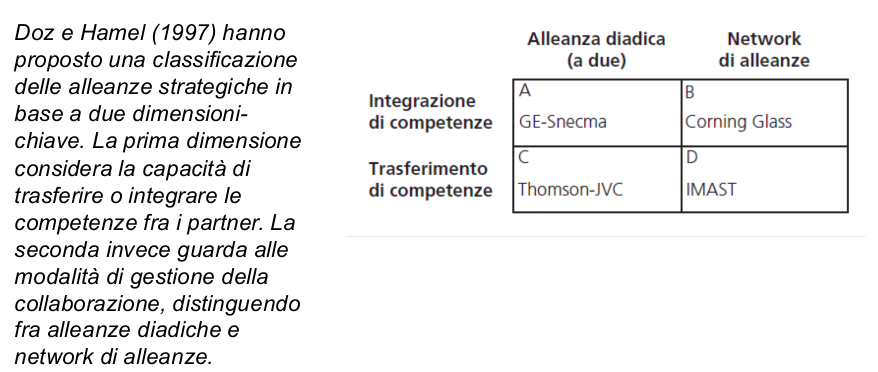
\includegraphics[scale=0.4]{images/allez_stra.png}
	\caption{Alleanza Strategica}
	\label{fig:Porter2}
\end{figure}
\begin{itemize}
\item Integrazione di competenze $\rightarrow$ l’azienda trasferisce ad una o più aziende un componente che
viene integrato nel prodotto da loro realizzato (es. Rolls-Royce produce motori per la Boeing che li
integra nel suo prodotto). Se il trasferimento riguarda due sole aziende si parla di alleanza diadica.
\item Trasferimento competenze $\rightarrow$ l’azienda trasferisce non soltanto il componente ma anche il know-
how che sta dietro la sua realizzazione (passaggio più complesso). Esso può riguardare due sole
imprese o un network di alleanze (es. Ducati che integra dai vari fornitori esterni).
La distinzione non è sempre così netta. 
\end{itemize}


\begin{enumerate}
\item  \textbf{Alleanze strategiche}: accordi di natura formale o informale fra
due o più partner allo scopo di collaborare per una finalità.
\item \textbf{Joint venture}: è una forma particolare di alleanza che richiede ai
partecipanti di adottare una struttura formale, quasi sempre una
nuova entità giuridicamente separata dotata di capitale proprio.
\item \textbf{Licensing}:è un accordo contrattuale che conferisce a
un’organizzazione (o a un individuo) i diritti d’uso di una proprietà
intellettuale di un’altra organizzazione, di norma in cambio di una
royalty.
\item \textbf{Outsourcing}:è una formula in base alla quale un’impresa
trasferisce all’esterno determinati processi piuttosto di realizzarli
al proprio interno.
\item \textbf{Organizzazioni di ricerca}: sono organizzazioni costituite per
favorire la collaborazione fra un gruppo di soggetti, per esempio
imprese ed enti pubblici di ricerca.
\end{enumerate}

\subsection{Alleanze e licensing per stabilire uno standard}
\begin{figure}[h!]
	\centering
	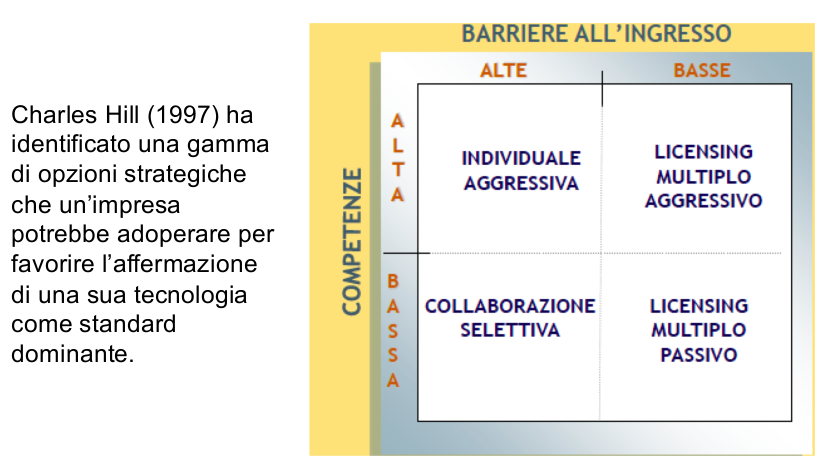
\includegraphics[scale=0.4]{images/licensing.png}
	\caption{Alleanza Strategica}
	\label{fig:Porter2}
\end{figure}

\begin{enumerate}
	\item Individuale – Aggressiva (evita collaborazioni; strategie di diffusione e politiche aggressive
	di prezzo)
	Se si genera un’innovazione e si vuole far affermare questa come dominant design, laddove
	ci siano competenze molto complesse ed alte barriere all’entrata è preferibile una strategia
	individuale. Essendo l’unico produttore c’è maggiore possibilità di affermazione di un
	dominant design poiché ci saranno pochi concorrenti nel futuro. Ciò conviene quando ci
	sono beni complementari e assenza di concorrenti competitivi.
	\item Collaborazione selettiva (alte barriere, basse competenze)
	Si stabilisce un’alleanza per promuovere uno standard, alleanza poiché c’è il rischio che un
	concorrente possa sviluppare la medesima tecnologia o una concorrente. Ciò conviene
	quando il partner è un potenziale concorrente (bassa competenza facilmente acquisibile
	dai concorrenti). L’impresa necessita di risorse in possesso dei concorrenti.
	\item Licensing multiplo aggressivo (tecnologia/conoscenza concessa in licenza)
	Viene trasferita la licenza di una conoscenza a molte imprese (non si sviluppa la conoscenza
	con altre aziende). Persegue strategie aggressive di posizionamento. Conviene in presenza
	di molti potenziali concorrenti (proprie per le basse barriere all’entrata) che potranno
	sviluppare tecnologie diverse.
	\item Licensing multiplo passivo (es. Microsoft, concede il sistema operativo in licenza a tutti i
	produttori di hardware)
	Viene concessa la licenza a tutti gli operatori interessati. Conviene quando ci sono molti
	concorrenti.
\end{enumerate}

\subsection{Scelta e controllo dei partner}
La collaborazione non è una strategia priva di rischi per cui la scelta dei partner giusti è
fondamentale. È difficile stabilire se le risorse fornite dai partner siano adeguate alla propria
impresa. Può anche accadere che qualcuno dei partner sfrutti il rapporto di collaborazione per
appropriarsi di conoscenze senza offrire nulla in cambio. Inoltre, poiché il management può
governare e mantenere sotto il controllo in modo efficace solo un numero limitato di
collaborazioni, l’efficacia di gestione diminuisce all’aumentare del numero di collaborazioni nelle
quali l’impresa è coinvolta.
Scaricato da Giulio Pilotto (pilotto.giulio@gmail.com)lOMoARcPSD|3519035
Il successo di una strategia di collaborazione dipende dai partner che sono stati scelti.
La compatibilità fra i partner può essere influenzata da diversi fattori. Questi fattori possono
essere ricondotti a due dimensioni:
La compatibilità delle risorse: fa riferimento alla potenziale disponibilità nei partner di
risorse che si prestano ad essere integrate e combinate in modo efficace nell’ambito di una
strategia per la creazione di valore. Le risorse dei partner possono essere complementari o
supplementari.
Compatibilità strategica, fa riferimento al grado di allineamento degli obiettivi e degli stili
imprenditoriali dei partner. Tali obiettivi non devono necessariamente coincidere, purché
possano essere perseguiti e raggiunti senza recare danno all’alleanza o agli altri partner.
Gli accordi di collaborazione di maggior successo mostrano meccanismi di governance e di
monitoraggio dei partner ben definiti. In molti casi le parti stipulano accordi contrattuali con
norme vincolanti allo scopo di assicurarsi che ciascun partner sia pienamente consapevole dei
propri diritti e doveri e possa ricorrere alle vie legali in caso di violazione dell’accordo. Nei contratti
si definiscono i seguenti punti:
Il contributo che ciascun partner si obbliga a fornire e a mettere a disposizione della
collaborazione in termini di risorse finanziarie, servizi, ecc.
Il grado di controllo di ciascun partner.
I tempi e i modi della distribuzione di quanto viene generato nel rapporto di collaborazione.
\section{Meccanismo di protezione dell'innovazione}
Nel formulare una strategia di innovazione, un elemento fondamentale è rappresentato dalla
definizione dei meccanismo di protezione delle innovazioni tecnologiche.
A volte, però, è nell’interesse dell’impresa non proteggere l’innovazione, perché incoraggiare altri
operatori (produttori e fornitori di beni complementari) a sostenere la nuova tecnologia può
determinare un più alto tasso di adozione e un processo rapido di diffusione, aumentando la
probabilità di acquisire la posizione di standard dominante.
\textbf{appropiabilità} (concetto opposto a quello di IMITABILITA’)  si intende la capacità
dell’impresa di acquisire e trattenere per sé le rendite generate dai propri processi innovativi. Il
grado di appropriabilità di un’innovazione è determinato dalla facilità e dalla rapidità con cui i
concorrenti riescono ad imitarla (tanto più aumento l’imitabilità tanto minore è la capacità di
appropriabilità). Il grado di imitabilità, a sua volta, è funzione sia della natura delle tecnologia
sviluppata sia dell’efficacia dei meccanismi di protezione adottate.
Se la base di conoscenze è tacita (difficilmente codificabile in documenti o formule) o socialmente
complessa è alquanto improbabile che i concorrenti riusciranno a imitarla o a riprodurla.
Tanto più l’innovazione si basa su conoscenze tacite tanto più l’appropriabilità è alta e l’imitabilità
è bassa.

Brevetti, marchi e copyright costituiscono tutti metodi di protezione della proprietà intellettuale
ma ciascuno è predisposto per la tutela di innovazioni differenti.
Un brevetto protegge un’invenzione; un marchio protegge parole o simboli distintivi della fonte di
provenienza e della proprietà di un bene; il copyright protegge il diritto dell’autore.

\subsection{Brevetti}

Sono delle nuove invenzioni che implicano un’attività inventiva e sono atte ad avere
un’applicazione industriale (valore economico). Il brevetto è una nuova conoscenza che viene
comunicata al fine di essere tutela dal punto di vista giuridico. Tutti i proventi derivanti da essa
sono da attribuire al titolare del brevetto. In mancanza di comunicazione non si può agire contro il
terzo che lo utilizza.
Cosa può essere brevettato?
\begin{itemize}
	\item Novità
	\item Un’innovazione che implichi un’attività inventiva, cioè non sia qualcosa di ovvio, ma
	originale (non possono essere brevettate le scoperte della natura)
	\item Tutto ciò che può avere un’applicazione industriale (che permette un ritorno economico);
	Sia sufficientemente descritta.
	\item Alla base del brevetto c’è la comunicazione della nuova conoscenza (più dettagli più tutela), spesso
	la descrizione del know-how non è abbastanza completa, ciò è causa di numerose battaglie di
	brevetto.
	\item Non possono essere brevettate le scoperte e le invenzioni contrarie all’ordine pubblico.
\end{itemize}

\subsubsection{Strategie Brevettuali}
Uno studio empirico ha messo in evidenza che la maggior parte degli inventori che brevettano preferisce descriverne il contenuto prima ancora che il brevetto venga concesso (disclosure anticipata).Questa scelta permette loro di publicizzare le caratteristiche e l’ambito di applicazione della loro invenzione.La disclosure attraverso la domanda di brevetto stabilisce la data da cui i depositanti possono godere dei primi, provvisori, redditi generati dai diritti di proprietà.
\begin{itemize}
\item Strategie agressive: patent trolling: attraverso una società, patenttroll,che detiene brevetti, una società può minacciare cause legali per strappare lucrose transazioni e ricattare altre imprese. 
\item Patentthicket: fitta ragnatela di brevetti incrociati e sovrapposti per competere senza cadere preda in una  causa in materia dib revetti intentata da imprese concorrenti
\end{itemize}

\subsection{Marchi}
Un \textbf{marchio commerciale} (o trademark) è costituito da una parola, una frase, un simbolo, un
disegno o qualsiasi elemento distintivo della provenienza di un bene. I marchi non riguardano il
know-how o la conoscenza dell’innovazione ma, soltanto il prodotto.
Un marchio di \textbf{servizio} (o service mark) è un marchio
che contraddistingue un fornitore di un servizio

\subsection{Copyright}
Il copyright è una forma di protezione applicabile alle opere soggette a diritto d’autore.L’autore ha il diritto esclusivo di utilizzare economicamente l’opera in ogni forma e modo (nei limiti fissati dalla legge), può rivendicarne la paternità e opporsi a qualsiasi uso che possa pregiudicare la sua reputazioneLa Convenzione di Berna stabilisce un livello minimo di protezione con copyright per tutti i Paesi che hanno aderito.

\subsection{Segreto Industriale }
Il segreto industriale è rappresentato da informazioni di proprietà
esclusiva di un’impresa, che restano ignote all’esterno dell’organizzazione
aziendale.
I segreti industriali non devono rispondere a tutti i rigorosi requisiti previsti
dalle leggi sui brevetti, consentendo la protezione di una più ampia classe
di attività.
L'inforamzione viene ocsnidreata segreto idnustriale se:
\begin{itemize}
	\item Genear unvantagigo distintivo per l'impresa in termini di rnedtia economica.
	\item Conserva il proprio valore rimanendo strettaetmne confidenziale
\end{itemize}

\subsection{Vantaggi della protezione}
\begin{itemize}
	\item   I sistemi proprietari consentono alle imprese di appropriarsi di maggiori rendite (solo
	l’impresa gode dell’appropriabilità).
	\item I profitti generati dall’innovazione possono essere reinvestiti nel miglioramento
	tecnologico.
	\item L’impresa potrebbe essere disposta a subire delle perdite di breve termine perché
	l’affermazione come disegno dominante garantirebbe flussi costanti e duraturi.
	o L’impresa può mantenere il controllo architetturale della tecnologia.
	\item I meccanismi di protezione dell’innovazione e la loro efficacia variano notevolmente a seconda del:
	\begin{itemize}
		\item Settore
		\item Tipologia di innovazione (prodotto, processo, ecc.)(si brevettano maggiormente le
		innovazioni di prodotto)
		\item  Contesto locale (differenze tra Nord e Sud Italia)
	\end{itemize}
\end{itemize}

\subsection{Sistemi Aperti Sistemi Chiusi}
I sistemi aperti permettono a tutti di poter utilizzare la conoscenza.
(caso Arduino, open-source community)
I sistemi proprietari (wholly proprietari system) sono basati sul possesso esclusivo della tecnologia
da parte dell’impresa e su una strategia di protezione.
Talvolta, è nell’interesse dell’imprese non proteggere l’innovazione, perché ciò può determinare
un più alto e un più rapido tasso di adozione e aumentarne la possibilità di divenire lo standard
dominante.
Nei sistemi aperti la tecnologia adottata non è protetta legalmente ed è liberamente accessibile ad
altri produttori.

Vantaggi
\begin{itemize}
	\item Una tecnologia aperta consente e favorisce un processo più rapido di diffusione e adozione
	della tecnologia.
	\item La diffusione della tecnologia senza barriere può favorire la disponibilità di beni
	complementari.
	\item Una tecnologia aperta può beneficiare degli sforzi di sviluppo operati in altre imprese.
\end{itemize}




Fattori che incentivano la scelta tra un sistema aperto o chiuso:
\begin{enumerate}
\item  Capacità di produzione, competenze di marketing e risorse di capitale.
\item  L’opposizione del settore alla tecnologia sole source (a livello di industria era lontana l’idea
di fare open - source, mentre era più facile sul software).
\item Il grado di controllo sui rischi di frammentazione (se la community ha il vantaggio di
migliorare e diffondere il prodotto, ha lo svantaggio di creare tanti prodotti diversi).
\end{enumerate}


In realtà la maggior parte delle tecnologie è riconducibile a situazioni intermedie tra i due sistemi.
Dietro il licensing c’è sempre un brevetto (in genere il brevetto ottimizza i profitti).
ECCEZIONE: nel caso in cui la domanda di mercato di un prodotto è troppo elevata rispetto alla
capacità produttiva dell’azienda, può convenire il licensing (la parte del mercato aggiuntiva è
coperta dai guadagni derivanti dal licensing).



 





\section{Conclusion}
``I always thought something was fundamentally wrong with the universe'' \citep{adams1995hitchhiker}

\bibliographystyle{plain}
\bibliography{references}
\end{document}
